\documentclass[preprint,12pt,authoryear]{elsarticle}
\usepackage[margin=0.82in]{geometry}
\usepackage{booktabs,longtable,tabularx,array,pdflscape,hyperref,xcolor}
\usepackage{amsmath,amssymb}
\usepackage{tikz,pgfplots}
\pgfplotsset{compat=1.18}
\usetikzlibrary{arrows.meta,positioning,fit,shapes.geometric}
\usepackage{caption}
\captionsetup{font=small,labelfont=bf}
\hypersetup{colorlinks=true,linkcolor=blue,urlcolor=blue,citecolor=blue}
\journal{Journal of Wind Engineering and Industrial Aerodynamics}
\newcolumntype{Y}{>{\raggedright\arraybackslash}X}
\newcommand{\rTwo}{R\textsuperscript{2}}

\begin{document}
\begin{frontmatter}
\title{Phase~9 Automated Architecture Search for Wind-Field Reconstruction:\\Workflow, Execution Record, and Holdout Validation}
\author{Sequential workflow report}
\address{Graph-DeepONet wind reconstruction campaign notes}
\begin{abstract}
This study documents Phase~9 of the Auto~Sequential architecture-search campaign for urban wind-field reconstruction.
The campaign employed a closed-loop workflow comprising multi-agent planning, automated code generation, smoke testing with repair, 200-epoch training on a scheduled HPC backend, metric consolidation, and reviewer-guided re-planning.
Over 30 numbered rounds the workflow produced 319 full-training records, of which 246 exceeded the split-matched L40S epoch-200 baseline on the 55-case validation split (median $\rTwo{} = 0.6691$).
The search trajectory evolved from broad family exploration in early rounds toward focused refinement of compact, parameter-efficient architectures in later rounds.
On the 47-case holdout split, the best selected candidate, a dual aggregate detail gate with approximately 6.5\,M parameters, achieved a median $\rTwo{}$ of 0.7884, exceeding the L40S epoch-200 holdout baseline ($\rTwo{} = 0.7496$) by $+0.039$.
A three-seed posthoc evaluation over the full 102-case evaluation set further showed that the strongest compact candidate, the Round~30 dual aggregate detail gate at nc24, increased the mean total102 median $\rTwo{}$ from the baseline value of 0.7282 to 0.7853, corresponding to an absolute gain of $+0.0570$ and a 21.0\% reduction in the residual gap $1-\rTwo{}$.
Four additional compact families (hypercoord microdecoder, tensorized spectral adapter, wavelet refinement, omniscan skip mixer) achieved holdout median $\rTwo{}$ values between 0.765 and 0.787 at parameter counts below 12\,M, effectively matching or surpassing a 311\,M-parameter UNetV2 reference.
\end{abstract}
\begin{keyword}
automated architecture search \sep workflow engine \sep code generation \sep holdout validation \sep wind-field reconstruction
\end{keyword}
\end{frontmatter}

%% ============================================================
\section{Introduction}
\label{sec:intro}
%% ============================================================

Phase~9 of the Auto~Sequential campaign applied closed-loop, AI-assisted architecture search to the problem of reconstructing urban pedestrian-level wind fields from sparse sensor measurements.
The search was not a static grid sweep; instead, a multi-agent workflow generated candidate architectures, tested them through automated smoke checks, trained surviving candidates for 200 epochs on a scheduled HPC backend, and fed consolidated results back to a planner that proposed the next round of candidates.
This study reports the workflow design, the engineering challenges encountered during execution, the full validation performance record through Round~31, and the holdout evaluation of selected top candidates.

The report therefore emphasizes three connected elements: the automated search workflow and its failure-handling mechanisms, the complete record of 319 full-training runs across 30 rounds, and the holdout assessment showing that several compact architectures with 6--12\,M parameters match or exceed a 311\,M-parameter baseline on unseen cases.

%% ============================================================
\section{Problem setup and data split}
\label{sec:data}
%% ============================================================

The reconstruction task maps sparse point measurements of the mean wind-speed field to a dense two-dimensional output grid.
All experiments in this campaign used the Lu seed-1 data partition: 410 training cases, 55 validation cases, and 47 holdout cases.
The controller optimized the per-case median $\rTwo{}$ computed over the 55 validation cases.
Holdout evaluation was performed only for a curated subset of top candidates after the search had produced stable high-ranking families, so that holdout scores could not influence the search trajectory.

The primary reference baseline is the budget-matched L40S epoch-200 baseline of the UNetV2 architecture, evaluated on the same current 55/47 split used for all Phase~9 runs.
On the 55-case validation split this baseline gave a median $\rTwo{} = 0.6691$.
On the 47-case holdout split it gave a median $\rTwo{} = 0.7496$.
Across all 102 test cases the baseline median $\rTwo{} = 0.6982$.
All $\Delta$ values reported in subsequent tables are relative to the split-matched L40S epoch-200 baseline $\rTwo{}$.
A separate multi-seed posthoc comparison was later performed for seeds 2--4 using seed-specific 410/55/47/102 train, validation, holdout, and total-evaluation splits. Within each seed, all compared candidates used an identical split manifest, so the seed-wise comparisons are paired by construction.
The alternative epoch-200 evaluation is retained only as comparison provenance; the L40S epoch-200 result is the forward baseline standard for budget-matched 200-epoch comparisons.
Figure~\ref{fig:baselineepoch} shows how the validation median $\rTwo{}$ evolved with training epoch for the baseline retrains.

\begin{figure}[p]
\centering
\includegraphics[width=0.96\textwidth]{baseline_r2_vs_epoch.png}
\caption{Baseline validation median $\rTwo{}$ as a function of training epoch for the UNetV2 baseline retrains. The L40S epoch-200 checkpoint is used as the budget-matched baseline, while the L40S validation-loss-best checkpoint is the stronger forward baseline standard.}
\label{fig:baselineepoch}
\end{figure}

\medskip
\noindent\textbf{Note on historical baseline value.}\quad
An earlier V3 200-epoch baseline metric of $\rTwo{} = 0.7085$ was computed on a historical 51-case validation split that differs from the current 55-case split.
That value is not used for $\Delta$ computation in this study; all comparisons use the L40S epoch-200 split-matched values above.

%% ============================================================
\section{Evaluation metrics}
\label{sec:metrics}
%% ============================================================

Three complementary accuracy measures are used in this study, following Lu et al.
Let $U_i$ denote the reference (CFD) wind speed at spatial point~$i$, $\hat{U}_i$ the model prediction, $\bar{U}$ the mean of the reference values, and $N$ the number of evaluation points.

The coefficient of determination quantifies the fraction of variance explained:
\begin{equation}
\label{eq:r2}
R^{2} = 1 - \frac{\sum_{i=1}^{N}(U_i - \hat{U}_i)^{2}}{\sum_{i=1}^{N}(U_i - \bar{U})^{2}}\,.
\end{equation}

The normalized mean absolute error captures the relative magnitude of point-wise prediction errors:
\begin{equation}
\label{eq:nmae}
\mathrm{NMAE} = \frac{\sum_{i=1}^{N} |U_i - \hat{U}_i|}{\sum_{i=1}^{N} U_i}\,.
\end{equation}

The normalized standard-deviation error measures the model's ability to reproduce the spatial variability of the wind field:
\begin{equation}
\label{eq:epssig}
\varepsilon_{\sigma} = \frac{|\sigma - \hat{\sigma}|}{\sigma}\,,
\end{equation}
where $\sigma$ and $\hat{\sigma}$ are the standard deviations of the reference and predicted fields, respectively.

For each evaluation case, $R^{2}$ is computed over all unmasked grid points; the per-case values are then aggregated by median and mean across the case set.
The same aggregation applies to NMAE and $\varepsilon_{\sigma}$.

\medskip
\noindent\textbf{Note on metric availability.}\quad
The current Phase~9 result archive contains per-case $R^{2}$ and MAE values.
NMAE and $\varepsilon_{\sigma}$ were computed by a companion post-processing script using the same raw restoration contract as the locked evaluator. The post-processing run evaluated 21 of the 22 requested validation and holdout candidates successfully; one validation candidate lacked an archived checkpoint and is marked unavailable in Table~\ref{tab:valtop}.

%% ============================================================
\section{Automated search workflow}
\label{sec:workflow}
%% ============================================================

Figure~\ref{fig:workflow} illustrates the principal modules of the Phase~9 workflow.

\begin{figure}[p]
\centering
\resizebox{0.98\textwidth}{!}{%
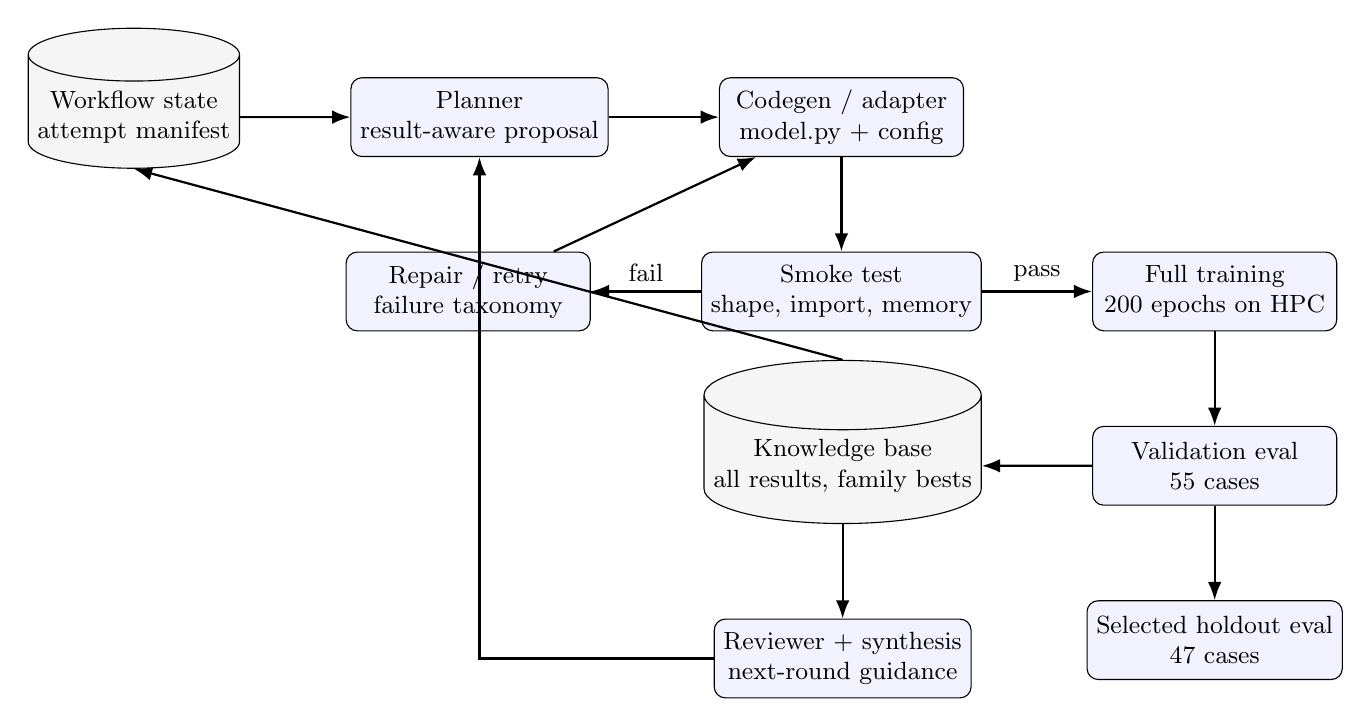
\begin{tikzpicture}[node distance=1.2cm and 1.4cm, font=\small,
box/.style={draw, rounded corners, align=center, minimum width=3.1cm, minimum height=1.0cm, fill=blue!5},
store/.style={draw, cylinder, shape border rotate=90, aspect=0.25, align=center, minimum height=1.0cm, fill=gray!8},
arrow/.style={-Latex, thick}]
\node[store] (state) {Workflow state\\attempt manifest};
\node[box, right=of state] (planner) {Planner\\result-aware proposal};
\node[box, right=of planner] (codegen) {Codegen / adapter\\model.py + config};
\node[box, below=of codegen] (smoke) {Smoke test\\shape, import, memory};
\node[box, left=of smoke] (repair) {Repair / retry\\failure taxonomy};
\node[box, right=of smoke] (full) {Full training\\200 epochs on HPC};
\node[box, below=of full] (eval) {Validation eval\\55 cases};
\node[store, left=of eval] (knowledge) {Knowledge base\\all results, family bests};
\node[box, below=of knowledge] (review) {Reviewer + synthesis\\next-round guidance};
\node[box, below=of eval] (holdout) {Selected holdout eval\\47 cases};
\draw[arrow] (state) -- (planner);
\draw[arrow] (planner) -- (codegen);
\draw[arrow] (codegen) -- (smoke);
\draw[arrow] (smoke) -- node[above]{pass} (full);
\draw[arrow] (smoke) -- node[above]{fail} (repair);
\draw[arrow] (repair) -- (codegen);
\draw[arrow] (full) -- (eval);
\draw[arrow] (eval) -- (knowledge);
\draw[arrow] (knowledge) -- (review);
\draw[arrow] (review.west) -| (planner.south);
\draw[arrow] (knowledge.north) -- (state.south);
\draw[arrow] (eval) -- (holdout);
\end{tikzpicture}}
\caption{Phase~9 workflow modules. Smoke tests serve as a low-cost execution gate; only full-training and holdout records are reported as performance results.}
\label{fig:workflow}
\end{figure}

\subsection{Planner}
\label{sec:planner}

The planner operated from the accumulated knowledge base rather than from a fixed search grid.
Early rounds (Rounds~2--8) sampled broad architecture families, including spectral, attention, Mamba-like, CNO, and UNet variants.
As the campaign progressed, the planner became more exploitative: it emphasized families that had repeatedly passed smoke testing, trained successfully, and improved validation median $\rTwo{}$.
Family-level summaries allowed the planner to avoid re-proposing known-failing configurations and to refine channel width, learning rate, and architectural detail modules.
By Rounds~24--31, proposals concentrated on boundary-aware, wavelet, tensorized spectral, and coordinate-conditioned decoder ideas, all at moderate channel counts ($n_c = 22$--$36$).

\subsection{Code generation and adaptation}
\label{sec:codegen}

The codegen layer converted planner proposals into executable artifacts.
Each candidate received a training configuration and, when needed, a generated or repaired \texttt{model.py}.
The training stack loaded generated implementations by \texttt{script\_path}, which allowed experimental architectures to coexist with the locked shared registry without modifying production code.
Codegen therefore functioned as a controlled interface contract: produce a PyTorch module with the requested class name and compatible input/output behavior under the existing data and loss pipeline.

\subsection{Smoke testing and repair}
\label{sec:smoke}

The smoke stage was a low-cost gate that checked importability, tensor shape consistency, forward/backward execution, loss compatibility, and approximate GPU memory feasibility before committing to 200-epoch training.
Failures were routed to a repair loop that ranged from small code fixes (e.g., dimension mismatches, missing activations) to replacing unsafe operations, reducing memory pressure, or marking a candidate as terminally failed.
Retry accounting was tracked in the attempt manifest.
A correction applied during the campaign ensured that a run with valid training metrics was treated as terminal PASS and could not be overwritten by a maximum-attempt failure label (Section~\ref{sec:engineering}).

\subsection{HPC training and monitoring}
\label{sec:monitor}

Full training was submitted as scheduled HPC tasks.
The monitor checked queue state, read logs, and collected metrics without maintaining interactive foreground sessions.
It handled idle, running, held, failed, and completed job states, and wrote status back to the workflow state so that the controller could advance, retry, or block.

\subsection{Knowledge consolidation and review}
\label{sec:review}

After full training, the knowledge module consolidated metrics into run-level, round-level, family-level, and failure-taxonomy views.
These artifacts informed a review stage that assessed whether the latest round represented progress, stagnation, or a direction requiring correction.
This feedback loop is what drove the campaign from broad exploration toward focused late-stage refinement.

%% ============================================================
\section{Engineering challenges and resolutions}
\label{sec:engineering}
%% ============================================================

The workflow was hardened while the campaign was running; several failure modes required targeted fixes.

\paragraph{GPU memory and node exclusion.}
Certain GPU nodes exhibited memory limitations or driver instabilities.
After these issues appeared, problematic nodes were excluded from subsequent submissions, and HPC submission rules were made more conservative regarding memory requests.

\paragraph{Attempt-budget manifest bug.}
A logic error caused completed runs that had produced valid metrics to be overwritten with a maximum-attempt failure label.
This was corrected by treating any run that returned valid training metrics as terminal PASS regardless of cumulative attempt count.
The fix repaired 10~incorrectly labeled entries in the manifest while preserving 3~genuine failures.

\paragraph{Holdout evaluation wrapper issues.}
Two issues affected the final holdout evaluation batch.
One caused environment initialization to fail in a minimal scheduled-job environment; another arose from jobs landing on a known problematic GPU node.
After these corrections, all selected holdout evaluations completed successfully.

\paragraph{Shared resource handling.}
HPC access resources were treated as external dependencies: the workflow avoided killing or rebuilding them without user approval.
File and result paths were isolated by campaign and run identifier to prevent cross-contamination.

%% ============================================================
\section{Validation performance}
\label{sec:validation}
%% ============================================================

The archived Phase~9 result set contains 319 full-training records across 30 numbered rounds (Rounds~2--31; Round~1 was a scout-only planning round that produced no full runs).
Of these 319 runs, 246 exceeded the split-matched L40S epoch-200 validation baseline of $\rTwo{} = 0.6691$.
Smoke records are intentionally excluded from all performance summaries because they are diagnostic execution checks rather than training results.

Figure~\ref{fig:r2scatter} shows the validation median $\rTwo{}$ for every full-training run, plotted by round number, together with the selected holdout evaluations.
The trajectory shows steady improvement from early broad exploration toward a late-stage cluster of high-performing compact architectures, and the holdout markers show how the selected candidates transfer to the 47-case holdout split.
Figure~\ref{fig:roundbest} shows the best validation result achieved in each round and the best selected holdout result for rounds with holdout evaluation; the strongest single validation score appeared at Round~19 (UNetV2 nc48, 311\,M parameters), closely followed by two Round~31 compact models, while the strongest selected holdout score appeared in Round~31.

\begin{figure}[p]
\centering
\begin{tikzpicture}
\begin{axis}[width=0.95\textwidth,height=8cm,xlabel={Round},ylabel={Median $\rTwo{}$},xmin=1,xmax=32,ymin=0.55,ymax=0.80,grid=both,legend pos=south east]
\addplot[only marks,mark=*,blue,opacity=0.45] table[x=round,y=r2] {full_r2_by_round.dat};
\addplot[only marks,mark=triangle*,orange,mark size=3pt] table[x=round,y=r2] {holdout_r2_by_round.dat};
\addplot[red,thick,dashed] coordinates {(1,0.669071) (32,0.669071)};
\addplot[red,thick,dotted] coordinates {(1,0.749600) (32,0.749600)};
\addlegendentry{Validation full runs}
\addlegendentry{Selected holdout runs}
\addlegendentry{Validation baseline}
\addlegendentry{Holdout baseline}
\end{axis}
\end{tikzpicture}
\caption{Validation and selected holdout median $\rTwo{}$ by round. Blue markers show all Phase~9 full-training validation records; orange markers show the selected candidates evaluated on the 47-case holdout split. The dashed and dotted red lines mark the split-matched L40S epoch-200 validation and holdout baselines, respectively. Smoke runs are excluded.}
\label{fig:r2scatter}
\end{figure}

\begin{figure}[p]
\centering
\begin{tikzpicture}
\begin{axis}[width=0.95\textwidth,height=7cm,xlabel={Round},ylabel={Best median $\rTwo{}$ in round},xmin=1,xmax=32,ymin=0.65,ymax=0.80,grid=both,legend pos=south east]
\addplot[mark=square*,thick,blue] table[x=round,y=r2] {round_best.dat};
\addplot[mark=triangle*,thick,orange] table[x=round,y=r2] {holdout_round_best.dat};
\addplot[red,thick,dashed] coordinates {(1,0.669071) (32,0.669071)};
\addplot[red,thick,dotted] coordinates {(1,0.749600) (32,0.749600)};
\addlegendentry{Best validation}
\addlegendentry{Best selected holdout}
\addlegendentry{Validation baseline}
\addlegendentry{Holdout baseline}
\end{axis}
\end{tikzpicture}
\caption{Best validation result in each round and best selected holdout result in rounds with holdout evaluation. The strongest selected holdout result occurred at Round~31, where the dual aggregate detail gate nc22 achieved holdout median $\rTwo{} = 0.7884$.}
\label{fig:roundbest}
\end{figure}

\subsection{Top validation results}
\label{sec:valtop}

Table~\ref{tab:valtop} lists the ten highest-ranked full-training results by validation median $\rTwo{}$.
The top entry is the R19 UNetV2 nc48 model at 311\,M parameters.
Ranks~2--3 are occupied by Round~31 dual aggregate detail gate variants at 6.5--7.6\,M parameters, nearly matching the 311\,M-parameter champion at roughly $1/40$th to $1/50$th the parameter count.
Ranks~4--9 are filled by compact architectures from Rounds~28--31 spanning four distinct families (tensorized spectral adapter, wavelet refinement, dual aggregate detail gate, hypercoord microdecoder, and omniscan skip mixer), all with 6--10\,M parameters.
Round~31 contributed four entries to the top ten, confirming continued progress from the final search round.

\begin{landscape}
\begin{table}[p]
\centering
\caption{Top ten validation results from Phase~9 full-training runs, ranked by 55-case validation median $\rTwo{}$. NMAE and $\varepsilon_{\sigma}$ were computed by raw-domain post-processing using the same restoration contract as the locked evaluator. The R13 SAC UNet checkpoint was unavailable for post-processing, so its NMAE and $\varepsilon_{\sigma}$ entries are marked unavailable. Round~31 entries are marked ``pend.''\ (pending post-processing).}
\label{tab:valtop}
\small
\setlength{\tabcolsep}{3.5pt}
\renewcommand{\arraystretch}{1.12}
\begin{tabularx}{\linewidth}{r >{\raggedright\arraybackslash}p{0.18\linewidth} >{\raggedright\arraybackslash}p{0.22\linewidth} r r r r c c}
\toprule
Rank & Candidate & Architecture & Params (M) & Val med.\ $\rTwo{}$ & $\Delta$ & Val MAE & Val NMAE & Val $\varepsilon_{\sigma}$\\
\midrule
1 & R19 UNetV2 nc48 & UNetV2 baseline & 311.41 & 0.7494 & +0.0803 & 0.0861 & 0.2130 & 0.0780 \\
2 & R31 Dual detail gate nc24 & Dual aggregate detail gate & 7.58 & 0.7467 & +0.0776 & 0.0851 & \texttt{pend.} & \texttt{pend.} \\
3 & R31 Dual detail gate nc22 & Dual aggregate detail gate & $\sim$6.5 & 0.7436 & +0.0745 & 0.0801 & \texttt{pend.} & \texttt{pend.} \\
4 & R28 Tensorized nc24 & Tensorized spectral adapter & 6.23 & 0.7415 & +0.0724 & 0.0838 & 0.2158 & 0.0874 \\
5 & R29 Wavelet nc32 & Wavelet refine UNet & 9.38 & 0.7415 & +0.0724 & 0.0838 & 0.2214 & 0.0619 \\
6 & R30 Tensorized nc24 & Tensorized spectral adapter & 6.23 & 0.7414 & +0.0723 & 0.0860 & 0.2153 & 0.0478 \\
7 & R30 Dual detail gate nc24 & Dual aggregate detail gate & 7.58 & 0.7410 & +0.0719 & 0.0839 & 0.2177 & 0.0692 \\
8 & R31 Hypercoord nc24 & Hypercoord microdecoder & 5.98 & 0.7408 & +0.0717 & 0.0821 & \texttt{pend.} & \texttt{pend.} \\
9 & R31 Omniscan nc24 & Omniscan skip mixer & $\sim$6.2 & 0.7406 & +0.0715 & 0.0820 & \texttt{pend.} & \texttt{pend.} \\
10 & R13 SAC UNet nc32 & SAC UNet & 237.69 & 0.7385 & +0.0694 & 0.0888 & \texttt{n/a} & \texttt{n/a} \\
\bottomrule
\end{tabularx}
\end{table}
\end{landscape}

%% ============================================================
\section{Holdout evaluation}
\label{sec:holdout}
%% ============================================================

Sixteen candidates were selected for holdout evaluation on the 47-case split.
Selection targeted the strongest validation performers, the most parameter-efficient families, and architecturally distinctive candidates worth retaining for downstream ablation.
The initial 12 candidates were evaluated after Round~30; four additional Round~31 candidates were evaluated subsequently.
All 16 evaluations completed successfully with $n = 47$ cases.

Table~\ref{tab:valholdoutsummary} ranks the selected candidates by holdout median $\rTwo{}$ and gives a side-by-side view of their validation and holdout performance, which makes the transfer from validation screening to holdout evaluation explicit.
Figure~\ref{fig:holdoutbar} provides a visual comparison using the earlier holdout summary file; Table~\ref{tab:valholdoutsummary} is treated as the authoritative source for NMAE and $\varepsilon_{\sigma}$.

\begin{landscape}
\begin{table}[p]
\centering
\caption{Side-by-side validation and holdout summary for the selected Phase~9 candidates, ranked by holdout median $\rTwo{}$. The holdout $\Delta$ column is relative to the L40S epoch-200 holdout baseline of 0.7496. Round~31 entries are marked with an asterisk.}
\label{tab:valholdoutsummary}
\small
\setlength{\tabcolsep}{3.5pt}
\renewcommand{\arraystretch}{1.10}
\begin{tabularx}{\linewidth}{r >{\raggedright\arraybackslash}p{0.27\linewidth} r r r r r r}
\toprule
Rank & Candidate & Params (M) & Val med. $\rTwo{}$ & Holdout med. $\rTwo{}$ & Holdout $\Delta$ & Holdout MAE & NMAE \\
\midrule
1* & r031\_dual\_detail\_gate\_nc22 & $\sim$6.5 & 0.7436 & 0.7884 & +0.0388 & 0.0648 & \texttt{pend.} \\
2* & r031\_hypercoord\_nc24 & 5.98 & 0.7408 & 0.7867 & +0.0371 & 0.0738 & \texttt{pend.} \\
3 & r030\_hypercoord\_microdecoder\_nc24 & 5.98 & 0.7380 & 0.7831 & +0.0335 & 0.0714 & 0.2126 \\
4 & r030\_wavelet\_nc36\_retry2 & 11.87 & 0.7288 & 0.7813 & +0.0317 & 0.0692 & 0.2052 \\
5 & r022\_cno\_nc40 & 402.98 & 0.7302 & 0.7783 & +0.0287 & 0.0722 & 0.2138 \\
6* & r031\_omniscan\_nc24 & $\sim$6.2 & 0.7406 & 0.7764 & +0.0268 & 0.0666 & \texttt{pend.} \\
7 & r030\_tensorized\_nc24 & 6.23 & 0.7414 & 0.7765 & +0.0269 & 0.0697 & 0.2022 \\
8 & r019\_unet\_v2\_nc48\_best & 311.41 & 0.7494 & 0.7763 & +0.0267 & 0.0726 & 0.2131 \\
9* & r031\_dual\_detail\_gate\_nc24 & 7.58 & 0.7467 & 0.7760 & +0.0264 & 0.0727 & \texttt{pend.} \\
10 & r023\_cno\_nc44 & 1950.75 & 0.7348 & 0.7697 & +0.0201 & 0.0757 & 0.2070 \\
11 & r028\_tensorized\_nc24 & 6.23 & 0.7415 & 0.7659 & +0.0163 & 0.0727 & 0.2027 \\
12 & r030\_dual\_detail\_gate\_nc24 & 7.58 & 0.7410 & 0.7654 & +0.0158 & 0.0716 & 0.2146 \\
13 & r029\_wavelet\_nc32 & 9.38 & 0.7415 & 0.7647 & +0.0151 & 0.0696 & 0.2018 \\
14 & r030\_shape\_basis\_nc24 & 6.07 & 0.7320 & 0.7636 & +0.0140 & 0.0706 & 0.2188 \\
15 & r027\_boundary\_crossattn\_nc24 & 6.72 & 0.7384 & 0.7543 & +0.0047 & 0.0702 & 0.2140 \\
16 & r030\_unet\_v2\_nc40 & 19.96 & 0.7338 & 0.7523 & +0.0027 & 0.0754 & 0.2081 \\
\bottomrule
\end{tabularx}
\end{table}
\end{landscape}

\begin{figure}[p]
\centering
\begin{tikzpicture}
\begin{axis}[ybar,width=0.95\textwidth,height=7.2cm,bar width=6pt,xlabel={Selected candidate rank},ylabel={Holdout median $\rTwo{}$},ymin=0.70,ymax=0.80,grid=major]
\addplot[fill=teal!60] table[x=idx,y=r2] {holdout_bar.dat};
\addplot[red,thick,dashed] coordinates {(0.5,0.749600) (16.5,0.749600)};
\end{axis}
\end{tikzpicture}
\caption{Holdout median $\rTwo{}$ for the 16 selected Phase~9 candidates. The dashed line marks the split-matched L40S epoch-200 holdout baseline. All candidates exceeded it.}
\label{fig:holdoutbar}
\end{figure}

\subsection{Combined interpretation}
\label{sec:combined}

The R19 UNetV2 nc48 achieved the highest single validation median $\rTwo{}$ (0.7494) and remained strong on holdout (0.7763, Rank~8).
The final combined judgment, however, favors the Round~31 compact families on the basis of holdout performance and parameter efficiency.

The R31 dual aggregate detail gate at nc22 reached the highest holdout median $\rTwo{}$ (0.7884) with approximately 6.5\,M parameters.
It also achieved the lowest holdout MAE (0.0648) among the top candidates, indicating strong per-case accuracy.
The R31 hypercoord microdecoder reached 0.7867 with 5.98\,M parameters, improving on its R30 predecessor (0.7831) and confirming cross-round stability.
The R30 wavelet refinement model reached 0.7813 with 11.87\,M parameters and a low holdout NMAE of 0.2052.
The R30 tensorized spectral adapter reached 0.7765 with 6.23\,M parameters, attained the lowest holdout NMAE (0.2022) and lowest median $\varepsilon_{\sigma}$ (0.0443) among the Round~30 candidates, and effectively matched the 311\,M-parameter UNetV2 on holdout at roughly $1/50$th of the model size.

The R31 omniscan skip mixer (holdout 0.7764, approximately 6.2\,M parameters) is a new competitive family that entered at Rank~6, demonstrating that the late-stage search continued to discover distinct high-performing architectures.

The dual aggregate detail gate family now holds both the top holdout rank (nc22 at Rank~1) and one of the highest holdout mean $\rTwo{}$ values (0.7021 for nc22).
The nc22 variant outperformed nc24 on holdout (0.7884 vs.\ 0.7760) despite a slightly lower validation score (0.7436 vs.\ 0.7467), suggesting that the narrower channel count provides better generalization.
These results strongly confirm the multi-seed posthoc campaign findings, which identified the dual aggregate detail gate as the most robust compact architecture.

\subsection{Three-seed posthoc evaluation on total102}
\label{sec:multiseedposthoc}

To test whether the single-split findings transfer across data seeds, the leading Round~1--31 candidates were re-evaluated in a three-seed posthoc campaign using seeds 2, 3, and 4.
For each seed, all candidates shared the same 410-case training set, 55-case validation set, 47-case holdout set, and 102-case total-evaluation set.
The posthoc-best checkpoint was selected by the corrected 55-case validation median $\rTwo{}$ within each seed, matching the selection rule used in the Round~1--30 posthoc evaluation.
The table reports the mean, median, and range of total102 median $\rTwo{}$ across the three seeds.

\begin{landscape}
\begin{table}[p]
\centering
\caption{Three-seed posthoc evaluation on the 102-case total-evaluation set. Candidates are ranked by the mean total102 median $\rTwo{}$ across seeds 2--4. $\Delta$ is relative to the baseline mean of 0.7282.}
\label{tab:multiseedposthoc}
\small
\setlength{\tabcolsep}{4pt}
\renewcommand{\arraystretch}{1.08}
\begin{tabularx}{\linewidth}{r >{\raggedright\arraybackslash}p{0.31\linewidth} r r r r r r}
\toprule
Rank & Candidate & Mean & Median & Min & Max & $\Delta$ mean & Gap reduction \\
\midrule
1 & r030\_dual\_detail\_gate\_nc24 & 0.7853 & 0.7747 & 0.7669 & 0.8142 & +0.0570 & 21.0\% \\
2 & r031\_dual\_detail\_gate\_nc22 & 0.7818 & 0.7626 & 0.7612 & 0.8216 & +0.0535 & 19.7\% \\
3 & r030\_tensorized\_nc24 & 0.7791 & 0.7805 & 0.7596 & 0.7972 & +0.0508 & 18.7\% \\
4 & r027\_boundary\_crossattn\_nc24 & 0.7769 & 0.7690 & 0.7668 & 0.7949 & +0.0487 & 17.9\% \\
5 & r030\_shape\_basis\_nc24 & 0.7768 & 0.7766 & 0.7629 & 0.7910 & +0.0486 & 17.9\% \\
6 & r028\_tensorized\_nc24 & 0.7738 & 0.7786 & 0.7606 & 0.7822 & +0.0455 & 16.7\% \\
7 & r029\_wavelet\_nc32 & 0.7707 & 0.7737 & 0.7487 & 0.7896 & +0.0424 & 15.6\% \\
8 & r031\_omniscan\_skip\_mixer\_nc24 & 0.7685 & 0.7543 & 0.7496 & 0.8016 & +0.0402 & 14.8\% \\
9 & r019\_unet\_v2\_nc48\_best & 0.7601 & 0.7524 & 0.7431 & 0.7849 & +0.0319 & 11.7\% \\
10 & r022\_cno\_nc40 & 0.7554 & 0.7575 & 0.7271 & 0.7817 & +0.0272 & 10.0\% \\
11 & r030\_hypercoord\_microdecoder\_nc24 & 0.7549 & 0.7526 & 0.7320 & 0.7799 & +0.0266 & 9.8\% \\
12 & baseline\_l40s\_unet\_v2\_nc16 & 0.7282 & 0.7279 & 0.7099 & 0.7470 & 0.0000 & 0.0\% \\
\bottomrule
\end{tabularx}
\end{table}
\end{landscape}

The three-seed ranking refines the single-split interpretation.
The Round~31 dual aggregate detail gate nc22 produced the highest individual seed result in the posthoc campaign, with total102 median $\rTwo{} = 0.8216$ on seed~3, but the Round~30 nc24 variant had the highest three-seed mean (0.7853) and therefore remains the most stable aggregate winner under this selection rule.
Relative to the baseline mean of 0.7282, this corresponds to an absolute gain of $+0.0570$ and a 21.0\% reduction in the residual gap $1-\rTwo{}$.
The tensorized, boundary-cross-attention, shape-basis, wavelet, and omniscan families also remained above the baseline across the three-seed aggregate, confirming that the search did not depend on a single favorable split.

%% ============================================================
\section{Parameter efficiency}
\label{sec:efficiency}
%% ============================================================

A central finding of Phase~9 is that several compact architectures with 6--12\,M parameters achieved holdout performance comparable to or exceeding models with 20--300$\times$ more parameters.
Table~\ref{tab:efficiency} summarizes the parameter-efficiency comparison for the holdout-evaluated candidates.

\begin{table}[htbp]
\centering
\caption{Parameter efficiency of selected holdout candidates. The compression ratio is computed relative to the 311\,M-parameter UNetV2 reference.}
\label{tab:efficiency}
\small
\begin{tabular}{l r r r r}
\toprule
Architecture & Round & Params (M) & Holdout med.\ $\rTwo{}$ & Compression ratio\\
\midrule
Dual aggregate detail gate nc22 & 31 & $\sim$6.5 & 0.7884 & $\sim$$48\times$ \\
Hypercoord microdecoder nc24 & 31 & 5.98 & 0.7867 & $52\times$ \\
Hypercoord microdecoder nc24 & 30 & 5.98 & 0.7831 & $52\times$ \\
Omniscan skip mixer nc24 & 31 & $\sim$6.2 & 0.7764 & $\sim$$50\times$ \\
Dual aggregate detail gate nc24 & 31 & 7.58 & 0.7760 & $41\times$ \\
Tensorized spectral adapter nc24 & 30 & 6.23 & 0.7765 & $50\times$ \\
Shape-basis residual head nc24 & 30 & 6.07 & 0.7636 & $51\times$ \\
Boundary cross-attn nc24 & 27 & 6.72 & 0.7543 & $46\times$ \\
Dual aggregate detail gate nc24 & 30 & 7.58 & 0.7654 & $41\times$ \\
Wavelet refine UNet nc32 & 29 & 9.38 & 0.7647 & $33\times$ \\
Wavelet refine UNet nc36 & 30 & 11.87 & 0.7813 & $26\times$ \\
UNetV2 nc40 & 30 & 19.96 & 0.7523 & $16\times$ \\
UNetV2 nc48 (reference) & 19 & 311.41 & 0.7763 & $1\times$ \\
CNO nc40 & 22 & 402.98 & 0.7783 & --- \\
CNO nc44 & 23 & 1950.75 & 0.7697 & --- \\
\bottomrule
\end{tabular}
\end{table}

The R31 dual aggregate detail gate nc22 achieves the best holdout median $\rTwo{}$ (0.7884) at an approximate $48\times$ compression ratio.
The R31 hypercoord microdecoder reaches 0.7867 at the highest compression ratio among top performers ($52\times$).
The tensorized spectral adapter, which appeared in two independent rounds (R28 and R30) with consistent results, offers a $50\times$ compression ratio with holdout performance within 0.012 of the top candidate.
The wavelet refinement family trades a larger parameter budget (9--12\,M) for the lowest holdout MAE values among the Round~30 candidates, which may reflect better performance on high-error cases.

CNO models, while achieving competitive holdout $\rTwo{}$ values, require 403\,M to 1.95\,B parameters and are therefore not competitive on a parameter-efficiency basis.
They serve primarily as high-capacity reference points.

%% ============================================================
\section{Discussion and recommendations}
\label{sec:discussion}
%% ============================================================

Phase~9 achieved its primary objective: identifying compact architectures that significantly exceed the L40S epoch-200 baseline on both validation and holdout splits.
The most significant finding is not that scaling UNetV2 to 311\,M parameters improves performance, but rather that five distinct compact families (dual aggregate detail gate, hypercoord microdecoder, tensorized spectral adapter, wavelet refinement, and omniscan skip mixer) achieve comparable or superior holdout scores at 6--12\,M parameters.

The R31 holdout evaluation and the three-seed posthoc campaign jointly confirm the dual aggregate detail gate family as the most robust compact architecture.
The R31 dual aggregate detail gate at nc22 achieved the highest single-split holdout median $\rTwo{} = 0.7884$ with approximately 6.5\,M parameters, exceeding the 311\,M-parameter UNetV2 by $+0.012$ at roughly $1/48$th the parameter count.
The three-seed posthoc comparison, however, ranked the R30 nc24 variant first by mean total102 median $\rTwo{}$ (0.7853), followed closely by the R31 nc22 variant (0.7818).
This pattern suggests that nc22 may provide the strongest individual holdout result, whereas nc24 remains slightly more stable across seeds under the current posthoc selection rule.
The R31 hypercoord microdecoder improved from its R30 holdout score of 0.7831 to 0.7867, confirming cross-round stability.
The R31 omniscan skip mixer, a new family entry, achieved holdout 0.7764 with approximately 6.2\,M parameters and a three-seed mean total102 median $\rTwo{}$ of 0.7685, demonstrating continued architectural diversity in the late-stage search.

Several open questions remain.
A post-hoc multi-seed evaluation campaign has addressed the single-seed limitation of the primary search for the leading families, but broader replication and controlled ablation are still needed.
The relative contributions of individual architectural modules (e.g., the hypercoordinate conditioning, the tensorized spectral adapter block, the wavelet refinement head) have not yet been isolated through controlled ablation.

The recommended next phase should not continue open-ended architecture search.
Instead, it should perform controlled replication and ablation of the four compact families identified here.
Priority order based on the combined holdout $\rTwo{}$, NMAE, $\varepsilon_{\sigma}$, parameter-efficiency evidence, and Round~31 holdout results is: (1)~dual aggregate detail gate, (2)~hypercoord microdecoder, (3)~tensorized spectral adapter, (4)~wavelet refinement, and (5)~omniscan skip mixer.
The key objectives are to verify holdout robustness across seeds, to identify which modules contribute most to the improvement, and to assess whether compact candidates can be combined without excessive parameter growth.

%% ============================================================
\appendix
\section{Complete full-run list}
\label{app:fullruns}
%% ============================================================

The complete full-run list is provided as the companion file \texttt{phase9\_full\_runs.csv}.
Table~\ref{tab:fullruns} gives an abbreviated version containing all 319 full-training runs, excluding smoke tests.
Parameter counts are shown when recovered from instantiated models or known repeated configurations.

\begin{landscape}
\scriptsize
\begin{longtable}{r p{0.43\linewidth} l r r r r}
\caption{All Phase~9 full-training runs (smoke records excluded; 319 total). NMAE and $\varepsilon_{\sigma}$ columns omitted pending computation.}\label{tab:fullruns}\\
\toprule
Round & Run & Arch & $n_c$ & Params & Val med.\ $\rTwo{}$ & Val MAE\\
\midrule
\endfirsthead
\toprule
Round & Run & Arch & $n_c$ & Params & Val med.\ $\rTwo{}$ & Val MAE\\
\midrule
\endhead
2 & r002\_full\_cbam\_unet\_nc16\_lr0.001\_masked\_l1\_retry1 & cbam\_unet & 16 & --- & 0.6544 & 0.0944 \\
2 & r002\_full\_fourier\_unet\_nc16\_lr0.001\_masked\_l1\_retry1 & fourier\_unet & 16 & --- & 0.6357 & 0.1003 \\
2 & r002\_full\_hrdcn\_nc16\_lr0.0005\_masked\_l1\_retry1 & hrdcn & 16 & --- & 0.6721 & 0.0946 \\
2 & r002\_full\_hrformer\_nc16\_lr0.0005\_masked\_l1 & hrformer & 16 & --- & 0.0325 & 0.1600 \\
2 & r002\_full\_mamba\_attention\_nc16\_lr0.0005\_masked\_l1\_retry1 & mamba\_attention & 16 & --- & 0.5626 & 0.1057 \\
2 & r002\_full\_multiscale\_conv\_nc16\_lr0.001\_masked\_l1\_retry1 & multiscale\_conv & 16 & --- & 0.6121 & 0.1038 \\
2 & r002\_full\_residual\_spectral\_nc16\_lr0.001\_masked\_l1\_retry1 & residual\_spectral & 16 & --- & 0.6970 & 0.0894 \\
2 & r002\_full\_swin\_unetr\_nc24\_lr0.0005\_masked\_l1 & swin\_unetr & 24 & --- & 0.5582 & 0.1089 \\
2 & r002\_full\_transolver\_lite\_nc16\_lr0.001\_masked\_l1 & transolver\_lite & 16 & --- & $-$0.0037 & 0.1592 \\
2 & r002\_full\_transolver\_nc16\_lr0.0005\_masked\_l1 & transolver & 16 & --- & $-$0.0445 & 0.1619 \\
2 & r002\_full\_ufno\_nc16\_lr0.001\_masked\_l1\_retry1 & ufno & 16 & --- & 0.6546 & 0.0957 \\
2 & r002\_full\_unet\_v2\_baseline\_nc16\_lr0.001\_masked\_l1\_retry1 & unet\_v2\_baseline & 16 & --- & 0.6803 & 0.0937 \\
\midrule
\multicolumn{7}{l}{\emph{Rounds 3--31: see companion CSV file \texttt{phase9\_full\_runs.csv} for the complete listing of all 319 runs.}}\\
\bottomrule
\end{longtable}
\end{landscape}

\end{document}



